\section{Evaluation}
\label{sec:evaluation}

In the first part of this section, we analyze different kinds of ontologies and datasets
and investigate the usability of the results proposed above.
In the second part, we evaluate the implementation of Algorithm~$\mathsf{A}_{\text{prc}}$
and compare it to the reasoning system RDFox.

\subsection{The Parallel Tractability of the LUBM Datasets and YAGO Ontologies}

In this part, we analyze two popular datasets, LUBM and YAGO, and show the relations
between these two datasets and the theoretical results regarding parallel tractability.

\textbf{LUBM}. In the Semantic Web community, LUBM
(The Lehigh University Benchmark) is proposed to
facilitate the evaluation of ontology-based systems
in a standard and systematic way.
In the latest version of LUBM,\footnote{http://swat.cse.lehigh.edu/projects/lubm/}
the core ontology contains 48 classes and 32 properties, used to describe the departments and the staff of
universities. By setting a different number of universities for an ontology-generator, users can get datasets of any size based on the core ontology.
%
The statements about properties in the LUBM core ontology, such as inverse property statements,
can be rewritten into the datalog rules of the form (R1), (R2) and (R3) in Table~\ref{tab:dhl}.
Most of the statements about classes can be rewritten into the datalog rules of the form (T1) and (T3)
in Table~\ref{tab:dhl}. Five axioms have, however, the form $A\sqsubseteq\exists R.B$,
which requires existentially quantified variables in the rule head when rewriting
the axiom into a logic rule: $A(x)\rightarrow\exists y(R(x,y)\wedge B(y))$ ($\tau$),
where a free variable $y$ is introduced. This kind of axiom is a general case of (T4) in Table~\ref{tab:dhl}
for which $A$ is actually replaced by the top concept $\top$.
Similarly to how we handle (T4), we can also eliminate the free variable $y$
in rule $\tau$ via Skolemization, i.e., by replacing the variable $y$ with a new constant $o_R^{A,B}$.
In this way, rule $\tau$ can be rewritten into $A(x)\rightarrow R(x,o_R^{A,B})\wedge B(o_R^{A,B})$.
If we only focus on the materialization task, the rewriting approach via Skolemization guarantees the
completeness and correctness \cite{GrauHKKMMW13}.
On the other hand, rule $\tau$ is not considered when using OWL RL reasoners to handle LUBM \cite{UrbaniKMHB12,WeaverH09}.
In summary, if the rewriting approach is used for the above kind of rule,
the materialization of a LUBM dataset can be handled by
Algorithm~$\mathsf{A}_{\text{prc}}$.


\textbf{YAGO}. The knowledge base YAGO\footnote{http://www.mpi-inf.mpg.de/home/}
is constructed from Wikipedia and WordNet. The latest version
YAGO3 \cite{MahdisoltaniBS15} has more than 10 million entities
(e.g., persons, organizations, cities, etc.)
and contains more than 120 million facts about these entities.

In order to balance the expressiveness and computing efficiency,
a YAGO-style language, called the \emph{YAGO model}, is proposed based on
a slight extension of RDFS \cite{SuchanekKW08}. The YAGO model defines
a set of properties: \texttt{domain, range, subClassOf, subRelationOf} and \texttt{type},
and a set of classes: \texttt{entity, class, relation} and \texttt{acyclicTransitiveRelation}.
The facts in the YAGO model are stated by triples, e.g., $(r_1,
\texttt{subRelationOf}, r_2)$,
which are similar to the RDFS statements.
A group of rules for reasoning over YAGO ontologies
is specified as follows \cite{SuchanekKW08}:
\begin{enumerate}[leftmargin=8ex,label=(\arabic*),ref=\arabic*]
  \item $(r,\texttt{domain}, c), (x, r, y) \rightarrow (x,
    \texttt{type}, c)$\label{yago:r1}
  \item $(r,\texttt{range}, c), (x, r, y) \rightarrow (y,
    \texttt{type}, c)$\label{yago:r2}
  \item $(c_1, \texttt{subClassOf}, c_2), (x, \texttt{type}, c_1)
    \rightarrow (x, \texttt{type}, c_2)$\label{yago:r3}
  \item $(r_1, \texttt{subRelationOf}, r_2), (x, r_1, y) \rightarrow
    (x, r_2, y)$\label{yago:r4}
  \item $(r, \texttt{type}, \texttt{acyclicTransitiveRelation}), (x,
    r, y), (y, r, z) \rightarrow (x, r, z)$\label{yago:r5}
\end{enumerate}

According to the semantics given to YAGO \cite{SuchanekKW08}, the built-in properties in YAGO,
i.e., \texttt{domain, range, subClassOf, subRelationOf} and \texttt{type} act in the same
way as the terms in RDFS statements of the form (1--5) in Table~\ref{tab:rdfs}, respectively.
In contrast to RDFS, YAGO also allows for defining
transitive properties using the
class \texttt{acyclicTransitiveRelation}; further, any fact in some YAGO ontology cannot be
described using blank nodes. By carefully checking the rules (\ref{yago:r1}--\ref{yago:r5}) for the reasoning over YAGO ontologies,
one can see that these rules can be rewritten into the datalog rules
of the form (T3),\footnote{Both of Rule (\ref{yago:r1}) and
Rule (\ref{yago:r2}) can be rewritten into (T3).} (T1), (R1) and (R3) in Table~\ref{tab:dhl}, respectively.
Based on the above analysis, any YAGO ontology can be expressed in DHL
and satisfies the simple-concept and the simple-role restrictions. We then have that,
for any well-constructed class of YAGO ontologies,
Algorithm~$\mathsf{A}_{prc}$ 
can handle all of the ontologies in the class.

In addition to LUBM and YAGO, we further investigate different kinds of ontologies and datasets
including benchmarks, real-world ontologies and datasets that can be
expressed in ontology languages.
These ontologies and datsets are collected from the Prot\'{e}g\'{e}
ontology
library,\footnote{http://protegewiki.stanford.edu/wiki/Protege\textunderscore
  Ontology\textunderscore Library}
Swoogle\footnote{http://swoogle.umbc.edu/} and the Oxford ontology library.\footnote{http://www.cs.ox.ac.uk/isg/ontologies/lib/}
Based on the analysis of these ontologies, we found that, ignoring imports, many of them
belong to $\mathcal{D}_{\textit{\text{dhl}}}$ or $\mathcal{D}_{\textit{\text{dhl}}(\circ)}$.
All of these investigated ontologies and the analysis results are available online.\footnote{https://github.com/quanzz/PT}


\subsection{Evaluating the Implementation of Algorithm~$\mathsf{A}_{\text{prc}}$}

In this part, we evaluate the implemented prototype system ParallelDHL
for DHL$(\circ)$ materialization based on
Algorithm~$\mathsf{A}_{\text{prc}}$. We also provide evaluation
results for the state-of-the-art reasoning system RDFox
\cite{MotikNPHO14}, which can also handle parallel ontology
materialization. Since RDFox is already a mature system, developed by
several people over several years, we only provide the results for
reference, as a direct comparison with our initial, not yet optimized
prototype is not possible.

\textbf{Datasets}.
We select eight ontologies from the data sources given in the previous subsection;
four of the eight ontologies belong to $\mathcal{D}_{\textit{\text{dhl}}(\circ)}$ and
the rest of them does not satisfy the simple-concept or the simple-role
restriction.
The chosen eight ontologies are real ontologies and are applied in different fields.
The basic information for these ontologies
is summarized in Table~\ref{tab:info}.

\begin{table}[htb]
\centering
\caption{Information about the test ontologies, where
  $|\mathcal{T}|+|\mathcal{R}|$ denotes the number of axioms occurring
  in the ontology, $|\mathcal{A}|$ denotes the number of assertions
  in the ABox and the last column states whether the
  ontology belongs to $\mathcal{D}_{\textit{\text{dhl}}(\circ)}$}
\begin{tabular}{>{\hspace*{5mm}}ccrrc<{\hspace*{5mm}}}
\hline
\textbf{Ontology Name} & \textbf{Field} &
                                          $|\mathcal{T}|+|\mathcal{R}|$
  & $|\mathcal{A}|$ & $\mathcal{D}_{\textit{\text{dhl}}(\circ)}$\\
\hline

Finance&finance&1,934&6,152&no\\

Molecule&chemistry&43&0&no\\

GrossAnatomy&anatomy&2,276&13&no\\

Skeleton&medicine&815&0&no\\

\hline

ChemistryPrimitive&chemistry&167&0& yes\\

FacebookOnto&social networking&185&28& yes\\

Mahabharata&literature&69&2,036& yes\\

Transportation&traffic&925&511& yes\\

\hline
\end{tabular}
\label{tab:info}
\end{table}

In order to compare ABoxes of a similar scale, we generate a limited
number of ABox assertions with respect to the TBoxes and RBoxes for
the test ontologies using the generation method proposed by
\citet{Elhaik98}.  For each test ontology, e.g., the Finance ontology,
we generate 5 new ontologies with different ABoxes, denoted
Finance-$i$ ($i\in\{1,2,3,4,5\}$). The index $i$ indicates that the
number of ABox assertions of Finance-$i$ is $i\times100,000$. We also
use the term ``Finance series" to denote the five generated ontologies
for the Finance ontology. The other test ontologies are processed
similarly.

\begin{table}[htb]
\centering
\caption{Analysis of the reasoning results, where the \emph{minimal time
  ratio} is the minimal reasoning time
of ParallelDHL divided by the minimal reasoning time of RDFox and the
\emph{average speedup} is $1/4 (T_1/T_2 + T_2/T_4 + T_4/T_6 + T_6/T_8)$,
 where $T_i$ is the reasoning time with $i$ threads allocated}
{\setlength{\tabcolsep}{6mm}
\begin{tabular}{crrrrr}
\hline
series & 1 & 2 & 3 & 4 & 5\\
\hline
\multicolumn{6}{c}{minimal time ratio}\\%[-1mm]
% \multicolumn{6}{c}{{\footnotesize minimal reasoning time
% of ParallelDHL/minimal reasoning time of RDFox}}\\
\hline
Finance&0.54&1.36&0.94&0.99&1.70\\
Molecule&0.94&0.79&0.96&0.98&1.07\\
GrossAnatomy&0.65&0.48&0.84&0.77&0.83\\
Skeleton&1.11&\textbf{3.08}&\textbf{3.03}&\textbf{3.04}&\textbf{2.75}\\
ChemistryPrimitive&1.29&1.54&1.68&1.14&0.93\\
FacebookOnto&\textbf{0.23}&\textbf{0.22}&\textbf{0.19}&\textbf{0.24}&\textbf{0.22}\\
Mahabharata&1.19&1.19&0.99&0.84&0.89\\
Transportation&0.24&0.52&0.51&0.65&0.49\\
\hline
\multicolumn{6}{c}{average speedup of ParallelDHL with increasing
  number of threads}\\%[-1mm]
% \multicolumn{6}{c}{{\footnotesize
%   $1/4 (T_1/T_2 + T_2/T_4 + T_4/T_6 + T_6/T_8)$,
%  where $T_i$ is the reasoning time with $i$ threads allocated}}\\
\hline
Finance&3.06&1.88&2.29&2.95&2.73\\
Molecule&1.04&1.24&1.13&1.07&1.05\\
GrossAnatomy&1.41&1.69&1.33&1.32&1.22\\
Skeleton&3.28&1.84&1.65&1.74&1.96\\
ChemistryPrimitive&\textbf{1.46}&\textbf{1.43}&\textbf{1.44}&\textbf{1.51}&\textbf{1.65}\\
FacebookOnto&\textbf{1.81}&\textbf{1.83}&\textbf{1.82}&\textbf{1.61}&\textbf{1.78}\\
Mahabharata&\textbf{1.41}&\textbf{1.46}&\textbf{1.51}&\textbf{1.47}&\textbf{1.56}\\
Transportation&\textbf{1.98}&\textbf{1.57}&\textbf{1.61}&\textbf{1.55}&\textbf{1.59}\\
\hline
\multicolumn{6}{c}{average speedup of RDFox with increasing
  number of threads}\\%[-1mm]
% \multicolumn{6}{c}{{\footnotesize
%   $1/4 (T_1/T_2 + T_2/T_4 + T_4/T_6 + T_6/T_8)$,
%  where $T_i$ is the reasoning time with $i$ threads allocated}}\\
\hline
Finance&1.01&1.04&1.13&1.11&1.19\\
Molecule&0.90&1.03&0.95&1.01&0.99\\
GrossAnatomy&0.87&0.99&0.94&0.96&0.98\\
Skeleton&1.13&1.01&1.06&1.08&1.08\\
ChemistryPrimitive&1.28&1.16&1.14&1.11&1.15\\
FacebookOnto&1.22&1.08&1.07&1.09&1.09\\
Mahabharata&1.24&1.07&1.13&1.10&1.12\\
Transportation&1.14&1.04&1.03&1.08&1.11\\
\hline
\end{tabular}
% \begin{tabular}{crrrrr}
% \hline
% series & 1 & 2 & 3 & 4 & 5\\
% \hline
% &0.54&1.36&0.94&0.99&1.70\\
% Finance&3.06&1.88&2.29&2.95&2.73\\
% &1.01&1.04&1.13&1.11&1.19\\
% \hline
% &0.94&0.79&0.96&0.98&1.07\\
% Molecule&1.04&1.24&1.13&1.07&1.05\\
% &0.90&1.03&0.95&1.01&0.99\\
% \hline
% &0.65&0.48&0.84&0.77&0.83\\
% GrossAnatomy&1.41&1.69&1.33&1.32&1.22\\
% &0.87&0.99&0.94&0.96&0.98\\
% \hline
% &1.11&\textbf{3.08}&\textbf{3.03}&\textbf{3.04}&\textbf{2.75}\\
% Skeleton&3.28&1.84&1.65&1.74&1.96\\
% &1.13&1.01&1.06&1.08&1.08\\
% \hline
% &1.29&1.54&1.68&1.14&0.93\\
% ChemistryPrimitive&\textbf{1.46}&\textbf{1.43}&\textbf{1.44}&\textbf{1.51}&\textbf{1.65}\\
% &1.28&1.16&1.14&1.11&1.15\\
% \hline
% &\textbf{0.23}&\textbf{0.22}&\textbf{0.19}&\textbf{0.24}&\textbf{0.22}\\
% FacebookOnto&\textbf{1.81}&\textbf{1.83}&\textbf{1.82}&\textbf{1.61}&\textbf{1.78}\\
% &1.22&1.08&1.07&1.09&1.09\\
% \hline
% &1.19&1.19&0.99&0.84&0.89\\
% Mahabharata&\textbf{1.41}&\textbf{1.46}&\textbf{1.51}&\textbf{1.47}&\textbf{1.56}\\
% &1.24&1.07&1.13&1.10&1.12\\
% \hline
% &0.24&0.52&0.51&0.65&0.49\\
% Transportation&\textbf{1.98}&\textbf{1.57}&\textbf{1.61}&\textbf{1.55}&\textbf{1.59}\\
% &1.14&1.04&1.03&1.08&1.11\\
% \hline
% \end{tabular}
}
\label{tab:expresult}
\end{table}

\textbf{The Experimental Results}.
We evaluated ParallelDHL and RDFox over the above eight ontology series.
The running environment is a DELL server with a
memory of 16 GiB and 4 cores.
For fairness, we set the same number of threads (i.e., 1,2,4,6 and 8 threads, respectively)
for ParallelDHL and RDFox in each experiment. The resulting reasoning
times\footnote{The experimental results can be found at https://github.com/quanzz/PT.} are
presented in the 16 line graphs (denoted by $lg1$,...,$lg16$) of Figure~\ref{fig:linegraph},
where the abscissa of each line graph records the numbers of ABox assertions,
the ordinate records the reasoning times (in milliseconds),
and each of the five curves in different colors denotes the trend of reasoning time with the
corresponding number of threads allocated (we use line-$k$ to denote the curve
corresponding to $k$ threads).

% We further process the collected data and fill the results in Table~\ref{tab:expresult}, where each cell corresponds
% to a test ontology (see the row label) and a newly generated ABox (distinguished by the column labels);
% the three values from above to below in each cell are: (1) \emph{the minimal time ratio} - the minimal reasoning time
% of ParallelDHL divided by the minimal reasoning time of RDFox;
% (2) \emph{the average speedup of ParallelDHL};\footnote{Suppose $T_i$ is the reasoning time with $i$ threads allocated,
% the average speedup is $\frac{1}{4}(\frac{T_1}{T_2}+\frac{T_2}{T_4}+\frac{T_4}{T_6}+\frac{T_6}{T_8})$.}
% (3) \emph{the average speedup of RDFox}.
% The minimal time ratio describes the performance of ParallelDHL by using RDFox as the baseline.
% The indicator speedup and its derived indicators are the most common tools used for measuring the capacity of parallelism \cite{MotikNPHO14,KazakovKS14,UrbaniKMHB12}.
% Here, we use the average speedup \cite{ichiyoshiK92} to describe the average capacity of parallelism with different
% threads allocated.
% In the following, we give the detailed analysis based on the contents in Figure~\ref{fig:linegraph} and Table~\ref{tab:expresult}.

We further process the collected data and fill the results in Table~\ref{tab:expresult}, where each cell corresponds
to a test ontology (see the row label) and a newly generated ABox
(distinguished by the series column labels).
The minimal time ratio describes the performance of ParallelDHL by using RDFox as the baseline.
The indicator `speedup' and its derived indicators are the most common tools used for measuring the capacity of parallelism \cite{MotikNPHO14,KazakovKS14,UrbaniKMHB12}.
Here, we use the average speedup \cite{ichiyoshiK92} to describe the average capacity of parallelism with different
threads allocated.
In the following, we give a detailed analysis based on the contents in Figure~\ref{fig:linegraph} and Table~\ref{tab:expresult}.

\textbf{Analysis of the Experimental Results}.
According to the theoretical results in Section~\ref{sec:ptonto},
materialization of the
ontologies not belonging to $\mathcal{D}_{\textit{\text{dhl}}(\circ)}$
(Finance, Molecule, GrossAnatomy and Skeleton)
may not be tractable in parallel. In other words,
parallel techniques may not work for improving the efficiency of materialization.
This is shown in the line graphs of Figure~\ref{fig:linegraph}.
We can see that, in the line graphs ($lg1$-$lg8$) of the ontology series
that do not belong to $\mathcal{D}_{\textit{\text{dhl}}(\circ)}$, the four lines, line-2, line-4, line-6 and line-8,
intersect to some degree. This is more obvious in the line graphs for
the Finance and GrossAnatomy
series. For example, in line graph $lg1$,
line-2 stays higher than line-6, but lower than line-4.
The intersection of lines indicates that reasoning time cannot
obviously be reduced with more threads allocated.
This is also supported by the results of the average speedups.
From Table~\ref{tab:expresult}, we can see that the average speedups of ParallelDHL and RDFox
for the ChemistryPrimitive, FacebookOnto, Mahabharata and Transportation series
are more stable compared with the other ones, i.e., with an average of
$1.4$ for ParallelDHL. This means that the reasoning time can be reduced on average
by $1.4$ times with two more threads allocated
for ParallelDHL, and, $1.1$ for RDFox. For the four ontology series
that do not belong to $\mathcal{D}_{\textit{\text{dhl}}(\circ)}$,
the average speedups have a higher volatility. For example,
the Finance and Skeleton series lead to high average speedups that reach up to $3$,
while, for the Molecule and GrossAnatomy series, the average speedups are even below $1$.
In summary, from the experiments on the test ontology series,
parallelism leads to a more effective improvement for materializing the ontology series
that belong to $\mathcal{D}_{\textit{\text{dhl}}(\circ)}$ compared
with the ones outside of this fragment.

By analyzing the experimental results of ParallelDHL and RDFox, we have that
ParallelDHL is competitive system despite not yet being highly optimized.
From Table~\ref{tab:expresult}, we can find that most of the minimal time ratios are close to $1$.
This means that the reasoning times of ParallelDHL are close to that of RDFox in parallel.
In particular, for the GrossAnatomy, FacebookOnto and Transportation series, ParallelDHL performs
much better than RDFox; therein, for materializing FacebookOnto-3, ParallelDHL
only requires one fifth of the minimal reasoning time of RDFox.
On the other hand, for most ontology series,
the average speedups of ParallelDHL are overall higher than that of RDFox.
The main difference between ParallelDHL and RDFox lies in that ParallelDHL applies
the optimizations designed for Algorithm~$\mathsf{A}_{\text{opt}}$ (see Section~\ref{sec:ptclass}).
The higher average speedups of ParallelDHL also verifies the validity of the optimizations
used in Algorithm~$\mathsf{A}_{\text{opt}}$.
One may note that ParallelDHL is on average 3 times slower than RDFox
when handling the Skeleton series.
The main reason is that the computation of the \texttt{rch} relations
requires a large amount of time and the situation of path twisting occurs in Skeleton series.
This makes the the optimization based on \texttt{rch} relations invalid as discussed
in Section~\ref{sec:ptonto}. {\color{red}What does the bold font in
  the table mean?}


\begin{figure}[htbp]
\begin{center}
\includegraphics[width=1.5\textwidth,angle=270]{fig-lineGraph.eps}
\caption{The line graphs of all experiments. The 16 line graphs are labeled by $lg1$,...,$lg16$ respectively.}
\label{fig:linegraph}
\end{center}
\end{figure}

\begin{figure}[htbp]
  \centering
  \begin{minipage}{.45\textwidth}
    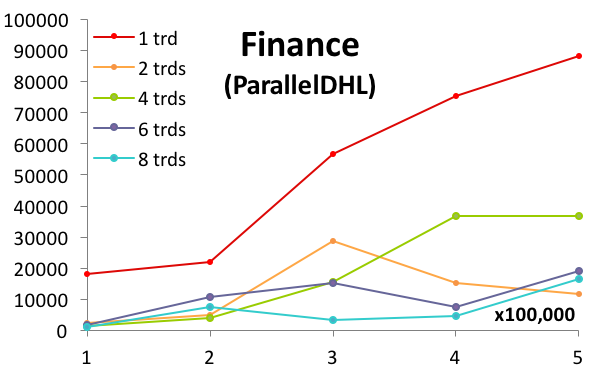
\includegraphics[width=\textwidth]{experimentalResults/1-Finance-simple}
    \subcaption{Finance (lg1)\label{fig:financepdhl}}
  \end{minipage}
  \begin{minipage}{.45\textwidth}
    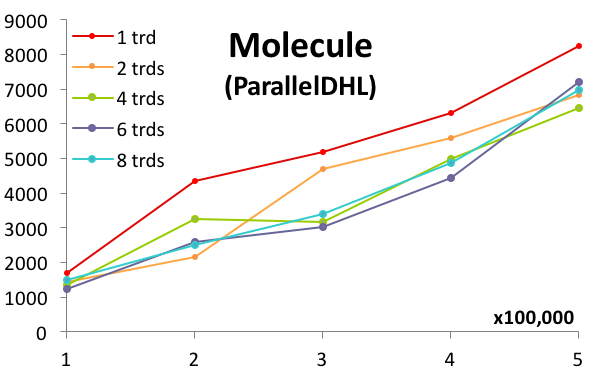
\includegraphics[width=\textwidth]{experimentalResults/2-molecule-simple}
    \subcaption{Molecule (lg3)\label{fig:moleculepdhl}}
  \end{minipage}\\
  \begin{minipage}{.45\textwidth}
    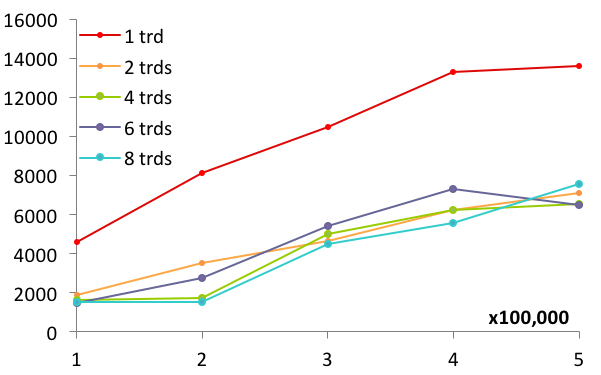
\includegraphics[width=\textwidth]{experimentalResults/3-NIF_GrossAnatomy-simple}
    \subcaption{GrossAnatomy (lg5)\label{fig:grossanatomypdhl}}
  \end{minipage}
  \begin{minipage}{.45\textwidth}
    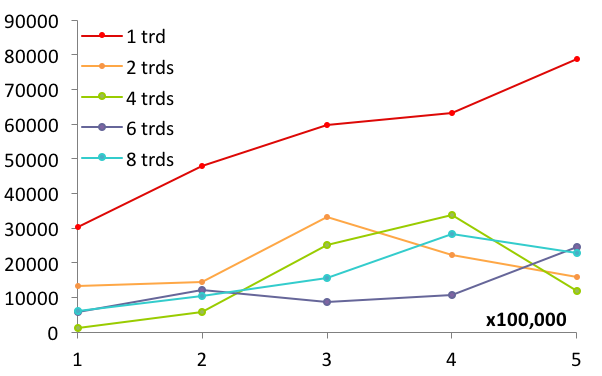
\includegraphics[width=\textwidth]{experimentalResults/4-skeleton-simple}
    \subcaption{Skeleton (lg7)\label{fig:skeletonpdhl}}
  \end{minipage}
  \caption{Materialization time in ms for ParallelDHL for the
    ontologies that do not belonging to $\mathcal{D}_{\textit{\text{dhl}}(\circ)}$.~\label{fig:eval}}
\end{figure}

\begin{figure}[htbp]
  \centering
  \begin{minipage}{.45\textwidth}
    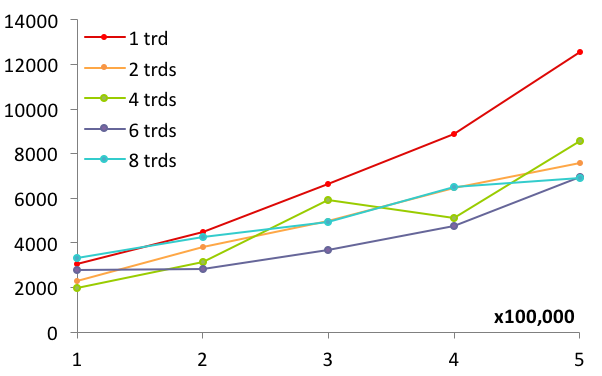
\includegraphics[width=\textwidth]{experimentalResults/1-Finance-rdfox}
    \subcaption{Finance (lg2)\label{fig:financerdfox}}
  \end{minipage}
  \begin{minipage}{.45\textwidth}
    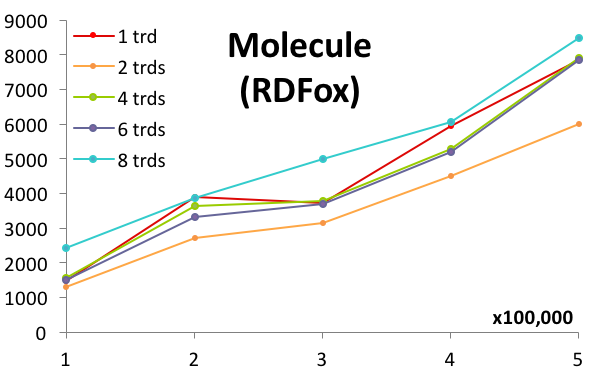
\includegraphics[width=\textwidth]{experimentalResults/2-molecule-rdfox}
    \subcaption{Molecule (lg4)\label{fig:moleculerdfox}}
  \end{minipage}\\
  \begin{minipage}{.45\textwidth}
    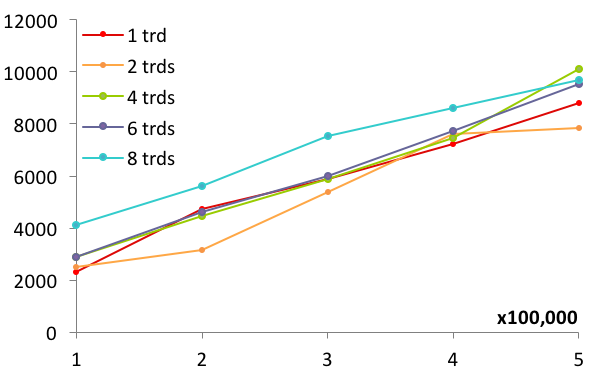
\includegraphics[width=\textwidth]{experimentalResults/3-NIF_GrossAnatomy-rdfox}
    \subcaption{GrossAnatomy (lg6)\label{fig:grossanatomyrdfox}}
  \end{minipage}
  \begin{minipage}{.45\textwidth}
    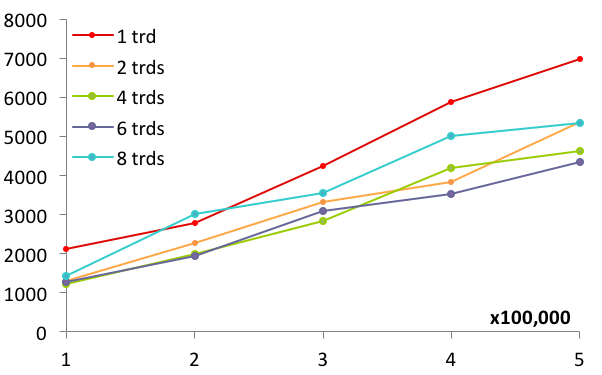
\includegraphics[width=\textwidth]{experimentalResults/4-skeleton-rdfox}
    \subcaption{Skeleton (lg8)\label{fig:skeletonrdfox}}
  \end{minipage}
  \caption{Materialization time in ms for RDFox for the
    ontologies that do not belonging to $\mathcal{D}_{\textit{\text{dhl}}(\circ)}$.~\label{fig:eval}}
\end{figure}

%%% Local Variables:
%%% mode: latex
%%% TeX-master: "parallel-tractability-J"
%%% End:
